 
 \documentclass{article}
\usepackage{amsmath,amscd,amsbsy,amssymb,latexsym,url,bm,amsthm}
\usepackage{epsfig,graphicx,subfigure}
\usepackage{enumitem,balance}
\usepackage{wrapfig}
\usepackage{mathrsfs, euscript}
\usepackage[usenames]{xcolor}
\usepackage{hyperref}
\usepackage[vlined,ruled,commentsnumbered,linesnumbered]{algorithm2e}

\newtheorem{theorem}{Theorem}[section]
\newtheorem{lemma}[theorem]{Lemma}
\newtheorem{proposition}[theorem]{Proposition}
\newtheorem{corollary}[theorem]{Corollary}
\newtheorem{exercise}{Exercise}[section]
\newtheorem*{solution}{Solution}
\theoremstyle{definition}
\hypersetup{hidelinks}
\definecolor{steelblue}{rgb}{0.27,0.51,0.71} 

\numberwithin{equation}{section}
\numberwithin{figure}{section}

\renewcommand{\thefootnote}{\fnsymbol{footnote}}

\newcommand{\postscript}[2]
 {\setlength{\epsfxsize}{#2\hsize}
  \centerline{\epsfbox{#1}}}

\renewcommand{\baselinestretch}{1.0}


\makeatletter \renewenvironment{proof}[1][Proof] {\par\pushQED{\qed}\normalfont\topsep6\p@\@plus6\p@\relax\trivlist\item[\hskip\labelsep\bfseries#1\@addpunct{.}]\ignorespaces}{\popQED\endtrivlist\@endpefalse} \makeatother
\makeatletter
\renewenvironment{solution}[1][Solution] {\par\pushQED{\qed}\normalfont\topsep6\p@\@plus6\p@\relax\trivlist\item[\hskip\labelsep\bfseries#1\@addpunct{.}]\ignorespaces}{\popQED\endtrivlist\@endpefalse} \makeatother



\begin{document}
\noindent

%========================================================================
\noindent\framebox[\linewidth]{\shortstack[c]{
\Large{\textbf{Homework 2}}\vspace{1mm}\\
CS420-Machine learning, Shikui Tu, Spring 2018}}
\begin{center}

\footnotesize{\color{steelblue}$*$ Name:Zhiwen Qiang  \quad Student ID:515030910367 \quad Email: qlightman@163.com}
\end{center}

\section{PCA algorithm}
\subsection{Algorithm 1}
\subsubsection{Pseudo code}
\begin{algorithm}[H]
\BlankLine
\SetKwInOut{Input}{input}
\SetKwInOut{Output}{output}
\caption{Algorithm 1}\label{Algorithm 1}
\Input{Data set $D=\{x1,\dots,x_N\},x_t\in R^{n*1},\forall t$ as input}
\Output{the first principal component $w$}
\BlankLine
Centralize the sample: $x_i \leftarrow x_i-\frac{1}{m}\sum_{i=1}^mx_i$;\\
Calculate the covariance matrix of the sample: $XX^T$;\\
Eigendecomposition of the covariance matrix: $XX^T$;\\
Obtain the corresponding eigenvector of the maximum eigenvalue.
\end{algorithm}
\subsubsection{Computational Details}
\begin{equation}
J(w)=\frac{1}{N}\sum^N_{t=1}||x_t-(x_t^Tw)w||^2\\
=x_t^Tx_t-w^T(x_tx_t^T)w
\end{equation}
Where $J(w)$ is the Mean Square Error (MSE).\\\\
Using Lagrange multiplier $\lambda$, we have 
\begin{equation}
L({x_t},w)=J({x_t},w)-\lambda(w^Tw-1)
\end{equation}
\begin{equation}
\frac{\partial J(w)}{\partial w}-\lambda\frac{\partial(w^Tw-1)}{\partial w}
=-2(\sum_xw)-\lambda*2w=0
\end{equation}
That is:
\begin{equation}
\sum_xw=(-\lambda)w
\end{equation}


\subsubsection{Advantages}
\begin{itemize}
\item It is an unsupervised method, which means that no information about groups is used in the dimension reduction.
\item It is the simplest of the true eigenvector-based multivariate analyses.
\end{itemize}

\subsubsection{Limitations}
\begin{itemize}
\item The results depend on the scaling of the variables. 
\item It assumes that the mapping function form high dimension to low dimension is linear, so it cannot reveal the intrinsic low dimension structure when dealing with non-linear mapping problem. As is shown in figure \ref{pca}, the result obtianed from PCA lost the original structure.
\begin{figure}[htbp]
	\centering
	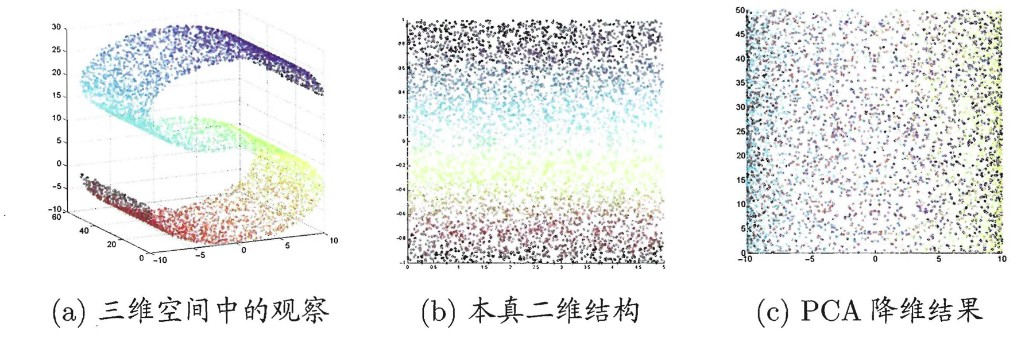
\includegraphics[width=10cm]{problem1/pca.jpg}
\caption{PCA results lack the original structrue.}
\label{pca}
\end{figure}

\end{itemize}
\subsection{Algorithm 2}
\subsubsection{Pseudo code}
\begin{algorithm}[H]
\BlankLine
\SetKwInOut{Input}{input}
\SetKwInOut{Output}{output}
\caption{Algorithm 2}\label{Algorithm 2}
\Input{Data set $X=\{x1,\dots,x_N\},x_t\in R^{n*1},\forall t$ as input}
\Output{the first principal component $w$}
\BlankLine
Calculate the distance matrix $D\in R^{m*m}$, where $dist_{ij}$ is the distance between sample $x_i$ to $x_j$;\\
Calculate $dist_{i.}^2$, $dist_{.j}^2$, $dist^2_{..}$ according to equation \ref{21begin} to \ref{2end}.\\
Calculate matrix $B$ according to equation \ref{2get}\\
Eigendecomposition of matrix $B$;\\
$\hat{\Lambda} $ is the diagonal matrix composed by the maximum eigenvalue $d$, $\hat{V}$ is the corresponding eigenvector matrix.\\
The first principal component $w=\hat{V}\hat{\Lambda}^{1/2}\in R^{m*1}$

\end{algorithm}
\subsubsection{Computational Details}
Let $B=Z^TZ\in R^{m*m}$, where $B$ is the matrix being dimensionality reduced, $b_{ij}=z_i^Tz_j$, we have:
\begin{equation}
\label{2beign}
dist_{ij}^2=||z_i||^2+||z_j||^2-2z_i^Tz_j
=b_{ii}+b_{jj}-2b_{ij} 
\end{equation}
After being centralize, it is easy to know:
\begin{equation}
\sum^m_{i=1}dist_{ij}^2=tr(B)+mb_{jj}
\end{equation}

\begin{equation}
\sum^m_{j=1}dist_{ij}^2=tr(B)+mb_{ii}
\end{equation}

\begin{equation}
\sum^m_{i=1}\sum^m{j=1}dist_{ij}^2=2mtr(B)
\end{equation}
Let:
\begin{equation}
\label{21begin}
dist_{i.}^2=\frac{1}{m}\sum^m_{j=1}dist^2_{ij}
\end{equation}

\begin{equation}
dist_{.j}^2=\frac{1}{m}\sum^m_{i=1}dist^2_{ij}
\end{equation}

\begin{equation}
\label{2end}
dist_{..}^2=\frac{1}{m^2}\sum^m_{i=1}\sum^m_{j=1}dist_{ij}^2
\end{equation}
From equation \ref{2beign} to \ref{2end}, we have:
\begin{equation}
\label{2get}
b_{ij}=-\frac{1}{2}(dist_{ij}^2-dist_{i.}^2-dist_{.j}^2+dist_{..}^2)
\end{equation}

\subsubsection{Advantages}
\begin{itemize}
\item It is a form of non-linear dimensionality reduction, which means it can reveal the intrinsic structure.
\item It is also an unsupervised method, which means that no information about groups is used in the dimension reduction.
\end{itemize}
\subsubsection{Limitations}
It require more training resources than Algorithm 1.

\section{Factor Analysis (FA)}
\subsection{E-step:}
\begin{equation*}
p^{old}(y|x)=\frac{G(y|0,I)G(x|Ay+\mu,\sigma^2I)}{G(x|\mu,AA^T+\sigma^2I)}
\end{equation*}
\begin{equation*}
E[y|x]=Wx \qquad W=A^T(AA^T+\sigma^2I)^{-1}
\end{equation*}
\begin{equation*}
E[yy^T|x]=I-WA+Wxx^TW^T
\end{equation*}
\subsection{M-step:}
\begin{equation*}
Q=\int p^{old}(y|x) \cdot \ln [G(y|0,I)G(x|Ay+\mu,\sigma^2I)]dy
\end{equation*}
In order to $max(Q(p^{old}(y|x),\Theta))$, we have:
\begin{equation*}
A^{new}=(\sum^N_{t=1}x_t(E[y|x_t])^T)(\sum^N_{t=1}E[yy^T|x_t])^{-1}
\end{equation*}
\begin{equation*}
\sigma^{2^{new}}=\frac{1}{Nd}Tr\bigg\{\sum^N_{t=1}\{x_tx_t^T-A^{new}E[y|x_t]x_t^T\}\bigg\}
\end{equation*}

\section{Independent Component Analysis (ICA)}
 The Central Limit Theorem, a classical result in probability
theory, tells that the distribution of a sum of independent random
variables tends toward a Gaussian distribution, under certain
conditions.

Thus, a sum of two independent random variables usually has a
distribution that is closer to Gaussian than any of the two original
random variables.
\begin{equation}
y=w^Tx=w^TAs=(w^TA)s=z^Ts
\end{equation}
$z^Ts$ is more Gaussian than any of the $s_j$. Therefore, we could take $w$ that maximizes
the non-Gaussianity.


\section{Causal discovery algorithms}
\subsection{Dataset description}
The data I use is a database with so far 108 two-variable cause-effect pairs 
created at Max-Planck-Institute for Biological Cybernetics in Tuebingen, Germany. It can be accessed via http://webdav.tuebingen.mpg.de/cause-effect/ . The datafiles are .txt-files and contain two variables, one is the cause and the other the effect. For every example there exists a description file where you can find the ground truth and how the data was derived. For example, in the pair0001.txt file, the two variables are altitude, temperature, the ground truth is that altitude is the cause, temperature is effect.
\subsection{Problem details}
The problem here is to find which is the cause and which the effect of the 108 two-variable cause-effect pairs.

\subsection{Algorithm details}
Here I use the algorithm described in Information-geometric causal inference, Daniusis et al. (2010); Janzing et al. (2012). The author of the paper first proposed two Postulate:

\begin{enumerate}
\item If $X \rightarrow Y$ , the distribution of $X$ and the function $f$
mapping $X$ to $Y$ are independent since they correspond
to independent mechanisms of nature.
\item Let $\varepsilon_X$ and $\varepsilon_Y$ define exponential families of “smooth” reference distributions for $X$ and $Y$ , respectively. Let
$u$ denote the projection of $p_X$ onto $\varepsilon_X$ and $u_f$ its image under f. If $X \rightarrow Y$, then
\begin{equation}
D(p_Y||\varepsilon_Y)=D(p_X||\varepsilon_X)+D(u_f||\varepsilon_Y).
\end{equation}
\end{enumerate}
The author then conclude that the consequence of Postulate 2 and the pos-
itivity of relative entropy is that if $X \rightarrow Y$,
\begin{equation}
C_{X \rightarrow Y}:=D(p_X||\varepsilon_X)-D(p_Y||\varepsilon_Y)<0.
\end{equation}
On the other hand, if $Y \rightarrow X$, We have
\begin{equation}
C_{Y \rightarrow X}:=D(p_Y||\varepsilon_Y)-D(p_X||\varepsilon_X)<0.
\end{equation}
Therefore, we have the defination of the Information Geometric Causal
Inference algorithm:\\\\
\textbf{Causal Inference method (IGCI):}Given $C_{X \rightarrow Y}$ ,
infer that $X$ causes $Y$ if $C_{X \rightarrow Y}<0$ , or that Y causes
X if $C_{X \rightarrow Y}>0$.



\subsection{Results}
\subsubsection{Results presented in the paper}
The author in the paper provide comparative results of
IGCI method (using two different reference measures)
and two other causal inference methods that are suit-
able for inferring the causal direction between pairs
of variables: the Additive Noise (AN) model and an implementation of the Post-NonLinear (PNL) model. The results in shown in table \ref{table1}.
\begin{table}[htbp]
\centering
\caption{Results for CauseEffectPairs data set (51 pairs)}
\label{table1}
\begin{tabular}{lll}
\hline
 Method& Decisions(\%) & Accuracy(\%)   \\ \hline
 IGCI (uniform)& 100& 78\\
 IGCI (Gaussian)& 100& 76\\
 AN (Gaussian)& 20& 100\\
 PNL& 82& 95
\end{tabular}
\end{table}
\subsubsection{Results produced myself}
It is worthy noting that the CauseEffectPairs data set is growing and I implemented the algorithm in a 108 two-variable cause-effect pairs.
The matlab code along with the dataset is in the 515030910367\_qiangzhiwen\_hw2 zip file. The environment I use is matlab 2015b, just execute the \textit{main.m} file and you can see the results.

\begin{table}[htbp]
\centering
\caption{Results for CauseEffectPairs data set (108 pairs)}
\label{table2}
\begin{tabular}{lll}
\hline
 Method& Decisions(\%) & Accuracy(\%)   \\ \hline
 IGCI (uniform,entropy)& 100& 65\\
 IGCI (uniform,integral)& 100& 65\\
 IGCI (Gaussian,entropy)& 100& 61\\
 IGCI (Gaussian,integral)& 100& 59
\end{tabular}
\end{table}
The results is shown in table \ref{table2}. I use two different reference measures and two different estimators of IGCI method to evaulate the results. We can see the accuracy is lower than the result in the paper. So I run the code on the inital dataset(51 pairs), the result is simailar compared to the paper. So I think the reason is that the additional pairs (57 pairs) have high noise level than the initial 51 pairs. 
\section{Causal tree reconstruction}
First we give a algorithm to reconstruct rooted trees. The detail in shown in algorithm \ref{Algorithm3}. 

\begin{algorithm}[H]
\BlankLine
\SetKwInOut{Input}{input}
\SetKwInOut{Output}{output}
\caption{Rooted trees reconstruction algorithm}\label{Algorithm3}
\Input{Data set $X=\{x1,\dots,x_N\},x_t\in R^{n*1},\forall t$ as input}
\Output{the first principal component $w$}
\BlankLine
$T_c=T_i$($T_c$ is a subtree of $T_i$ to which $x_{i+1}$ is to be added. It becomes progressively smaller by eliminating those sections of $T_i$ known not to contain $x_{i+1}$)\\
$s:=$ the number of leaves in $T_c$.\\
\If {$s=2$}{let $v$ be the root of $T_c$ and $x_j$,$x_k$ its two leaves.}
\If{$s>2$}{select as $v$ any node of $T_c$ for which $\frac{s}{k+1}<des(v)<\frac{sk}{k+1}$ and let $x_j,x_k$ be two leaves whose common ancestor is $v$}
Ask for the leader of the triple $(x_{i+1},x_j,x_k)$.
\If{$s>2$}{return to 1}
Define a partition of $T_c$ into two subtrees: $T_{c1}$ rooted at $v$ with all the descendants of $v$ and $T_{c2}=T_c-T_{c1}$ in which $v$ is considered a leaf.
\If{$x_{i+1}$ is the leader of $(x_{i+1},x_j,x_k)$}{set $T_c=T_{c2}$}
\If{there is no leader}{$T_c=T_{c1}$ from which the two sons of $v$ whose descendants are $x_j$ and $x_k$ are removed with all their descendants.}
\If{$x_j$ or $x_k$ is the leader}{set $T_c=$ the subtree of $T_{c1}$ rooted at that son of $v$ which is the ancestor of $x_k$ or $x_j$.}
\If{$s=2$}{return to 1}
\If{$x_j$ or $x_k$ is the leader}{add a new node on the edge of $x_k$ or $x_j$, and make it the father of $x_{i+1}$.}
\If{$x_{i+1}$ is the leader}{add a new root and make $x_{i+1}$ and the old root $v$ its sons.}
\If {there is no leader}{make $x_{i+1}$ a son of $v$.}
return to 1
\end{algorithm}


Then we prove that the rooted-tree proceduce can be adapted to unrooted trees as well. 

Let $T$ be an unrooted tree in which the degree of every node is at least three, and let $u,v,w,x$ be any quadruple of leaves. We say that $x$ pairs with $u$ relative to $(v,w)$ if the path from $x$ to $u$ is edge-disjoint relative to the path form $v$ to $w$.

Remove a leaf $x$ of $T$ and examine the remaining tree $T_1$ as rooted at the node $x_1$ with which $x$ is adjacent in $T$. Then we can use algorithm \ref{Algorithm3} to reconstruct $T_1$ rooted at $x_1$  and finally add $x$ as a son of $x_1$ to obtian the unrooted tree $T$.



%========================================================================
\end{document}
